\documentclass[11pt]{article}
\usepackage[margin=.85in]{geometry}
\usepackage{amsmath,amssymb,booktabs,graphicx,hyperref,placeins,microtype}
\hypersetup{colorlinks=true,linkcolor=blue!50!black,urlcolor=blue!50!black}
\setlength{\parindent}{0pt}\setlength{\parskip}{5pt}
\title{A nonadvective Gamma driver with an adapting reference\\\large Spherical implementation, boundary tests, and comparison}
\author{Isolated numerical experiment}
\date{27 October 2026}
\begin{document}\maketitle
\begin{abstract}The proposed bulk equations and their characteristic speeds are implemented and independently checked. Exact spherical nullness and the new driver compatibility hold to floating-point precision in the tests. The first incoming-characteristic boundary discretization nevertheless fails consistency with the metric-reconstructed connection constraint and has reproducible growing numerical modes. The short pulse and puncture tests fail the scri-numerator guard, so no qualified $100M$ result is obtained for this implementation, and no late-time improvement in horizon drift or settling is established. The completed coarse advective reference supplies the comparison baseline.\end{abstract}

\section{Candidate and controlled comparison}
The proposed shift uses the independent evolved Z4 connection:
\begin{align}
 \partial_t\beta&=\mu_\Gamma\Lambda-\eta_D(\beta-b),&
 \partial_t b&=\sigma(\beta-b).
\end{align}
The initial reference is the initial shift. The direct control has $\eta_D=\sigma=0$; the adaptive candidate has $\eta_D=1$, $\sigma=0.1$ in coordinate-time units. Both retain the full spherical metric, the existing telegrapher lapse with its $\chi$ and lapse attenuation, and the configurable physical lapse floor $10^{-10}$. The old shift advection, explicit $-r$ source, and $1/\Omega$ restoration are absent. Minkowski data $\beta=b=-r$, $\Lambda=0$ are an exact continuum equilibrium. For positive $\eta_D,\sigma$, stationarity requires $b=\beta$ and $\Lambda=0$; the final shift is not anchored to its initial value.

The main comparison uses $N=257$, the same wormhole data and initial elliptic shift as the completed advective control, grid stretch zero with the existing outer mapping collar, KO8 coefficient $0.5$, compact Z4 damping strength $8$, and $\Delta t/h=0.025$. The mass is $M=1/3$. The aligned duration target is coordinate $t=33.3333984375$, or $100.0002M$. Native equations, numerical sources, and the library binding were checked against the preserved reference. No existing worktree or job was changed.

A short diagnostic replay uses the unchanged frozen advective code and exactly recovers its completed coordinate-$0.2$ state and compensated-update array, bit for bit. It supplies the missing common snapshots through $0.45M$ in a new output directory. This is a sampling control on a successful interval; the original trajectory is untouched.

The predeclared low-resolution mass criteria are peak relative drift and final absolute relative error below $10^{-3}$. Each exterior constraint time RMS is compared separately with twice the matched advective value. Reduced horizon-coordinate drift means an absolute least-squares slope over the final $20M$ below half the advective slope. Field time derivatives, the reference gap, and connection residuals are also required to assess settling. A flat coordinate horizon alone is insufficient. These criteria are comparisons at finite resolution, not convergence criteria.

\section{Characteristic speeds and coefficient}
For the derivative reduction
\[
 U=(\chi_r,g_r,A_{rr},p/\Omega,\Theta/\Omega,\Lambda,\alpha_r,\beta_r,B_r),
 \qquad \partial_tU=L\,\partial_rU+\cdots,
\]
coordinate characteristic speeds are $-\operatorname{eig}(L)$. Exact symbolic factorization gives
\begin{align}
 \det(zI-L)={}&(z-\beta)
 \big[(z-\beta)^2-\alpha^2\chi/g\big]^2
 \big[(z-\beta)^2-c_L^2\big]\nonumber\\
 &{}\times\big[z^2-\beta z-4\mu_\Gamma/(3g)\big],\\
 c_L^2={}&\chi F/g+\eta\chi\kappa w^2/\tau .
\end{align}
Thus the proposed shift speeds are
\[
 v_\pm=-\frac{\beta}{2}\pm\frac12
       \sqrt{\beta^2+\frac{16\mu_\Gamma}{3g}}.
\]
The reference variable supplies an additional zero-coordinate-speed mode. A sufficient separation from both advected lapse speeds is
\[
 \frac{4\mu_\Gamma}{3g}>c_L^2+|\beta|c_L .
\]
It also separates the light speeds for the retained slicing. The outer coefficient
\[
 \mu_{\rm outer}=\frac{3g}{4}(2c_L^2+\beta^2)
\]
leaves the strictly positive margin $c_L^2+\beta^2-|\beta|c_L$ for $c_L>0$. A C7 collar blends constant bulk strength $4$ into this value between $r=0.8$ and $0.9$. The margin of the actual blend is evaluated at every stage. Exact eigenspaces reproduce the defective normalized-scri coefficient $3/2$ and the complete coefficient $9/4$. These scalar checks do not establish 3D or singular-endpoint well posedness.

\section{Incoming boundary implementation and its limitations}
Every stage and accepted state reconstructs
\[
 \beta=G=-\alpha\sqrt{\chi/g},\qquad
 G_t=\frac G2(\chi_t/\chi-g_t/g)
\]
with the fixed lapse clock. The new compatibility condition is
\[
 \mu_\Gamma\Lambda-G_t-\eta_D(G-b)=0 .
\]
It cannot be replaced by the old auxiliary-driver trace.

For the incoming eigenvalue
$\lambda=(\beta+\sqrt{\beta^2+16\mu_\Gamma/(3g)})/2>0$,
an exact right eigenvector normalized by $\delta\Lambda=1$ has
\[
 (\delta\chi_r,\delta g_r,\delta\Lambda,\delta\beta_r)
 =(-\chi g/2,\ g^2,\ 1,\ \mu_\Gamma/\lambda),
\]
with all other components zero. In particular
$\delta(\Lambda-V)=\delta\Lambda-\delta g_r/g^2=0$.
The implementation projects this complete incoming combination to satisfy the driver relation, leaving frozen outgoing and tangent amplitudes intact in that augmented first-order jet. It does not independently set $\Lambda=0$.

Three independent endpoint first derivatives are evolved using endpoint derivatives of the corresponding total-field rates. Their differences from ordinary finite-difference derivatives are measured as reduction defects. This additional numerical boundary construction requires its own stability test. Perturbed-metric tests verify projection idempotence, the incoming-vector identity, nullness, and compatible rates to floating-point precision.

The initial algebraic checks were too narrow to establish the requested physical outgoing-constraint preservation. A finite counterexample changes the reference endpoint while holding the metric values fixed. The projection changes the independent metric derivative together with $\Lambda$, so its augmented-jet constraint is preserved; the derivative reconstructed from the metric values does not change, however, and the corresponding physical discrete connection constraint changes by $g\,\delta\Lambda/2$. Thus this first boundary attempt fails reduction consistency and is not admitted as a compliant outgoing-constraint-preserving implementation of the proposed gauge. Both constraint definitions are retained in the diagnostics below, with the metric-reconstructed definition used for the primary comparison.

The native scri numerator limits and regularity traces remain approximate penalties. They include $\chi-g$, the shear-like trace $A_{rr}-g_r/6+2\chi_r/3$, $p$, $\Theta$, and $\Lambda-V$. The raw lapse-clock compatibility is recorded before imposing its zero rate. The shear-like trace varies along the incoming direction by $-g^2/6-\chi g/3$; imposing it as an extra arbitrary exact incoming datum would require a compatibility argument. Exact nullness, approximate regularity, and a well-posed boundary problem are distinct claims.

\section{Independent implementation and stability tests}
The discrete Minkowski RHS at $N=65$ has maximum magnitude $3.3\times10^{-12}$. Independent bulk identities confirm the requested nonadvective equations and the absence of the old reference forces. Native Einstein, lapse, and telegrapher rates match the advective implementation bitwise away from the modified boundary. One hundred randomized scalar-symbol checks have complete eigenspaces for the tested separated states.

The full constrained RK-step map was linearized around Minkowski equilibrium at two perturbation sizes. This includes all stage projections. Its spectral radius exceeds one for both new configurations at $N=25,33,65$; halving the differentiation perturbation reproduces the result. The matched advective $N=33$ map has spectral radius one. The dominant new modes are concentrated near the outer boundary, including when only physical-state variables are used to measure their localization.

\begin{figure}[htbp]\centering
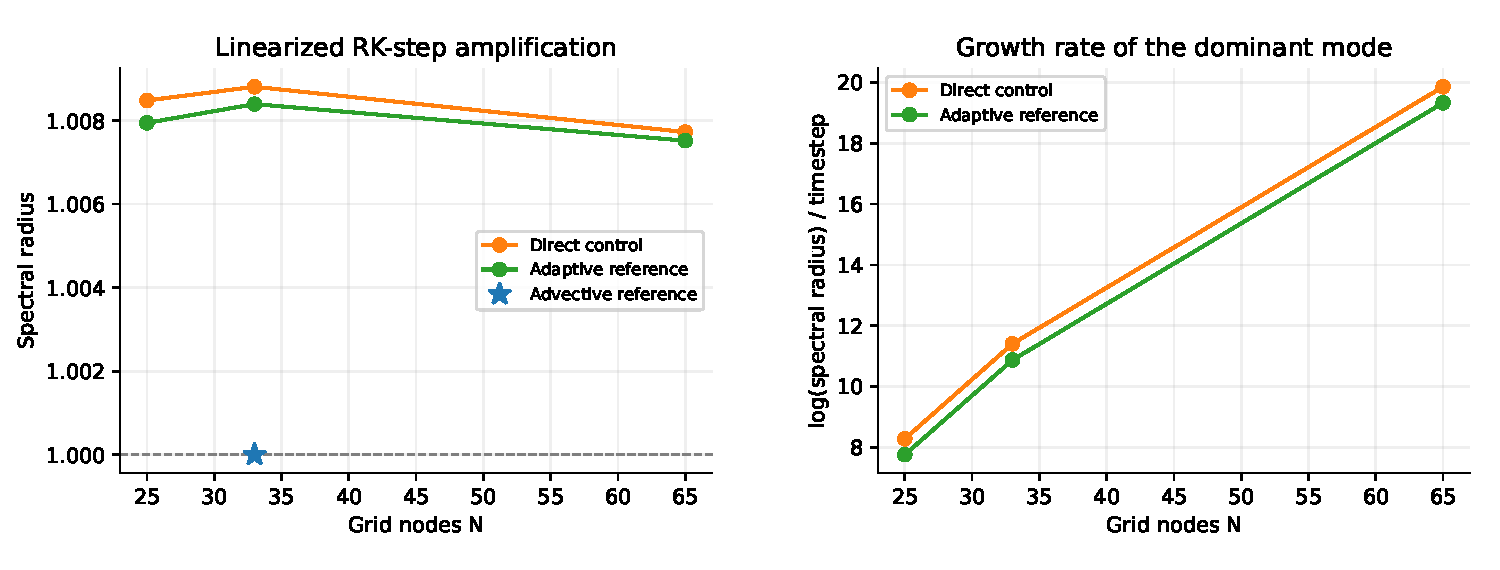
\includegraphics[width=\linewidth]{figures/linear-growth.pdf}
\caption{Independent full-step linearization at fixed CFL. Growth is a property of the tested discretization and background; this is not a nonlinear evolution or a proof that the continuum bulk gauge is impossible.}
\end{figure}
\begin{figure}[htbp]\centering
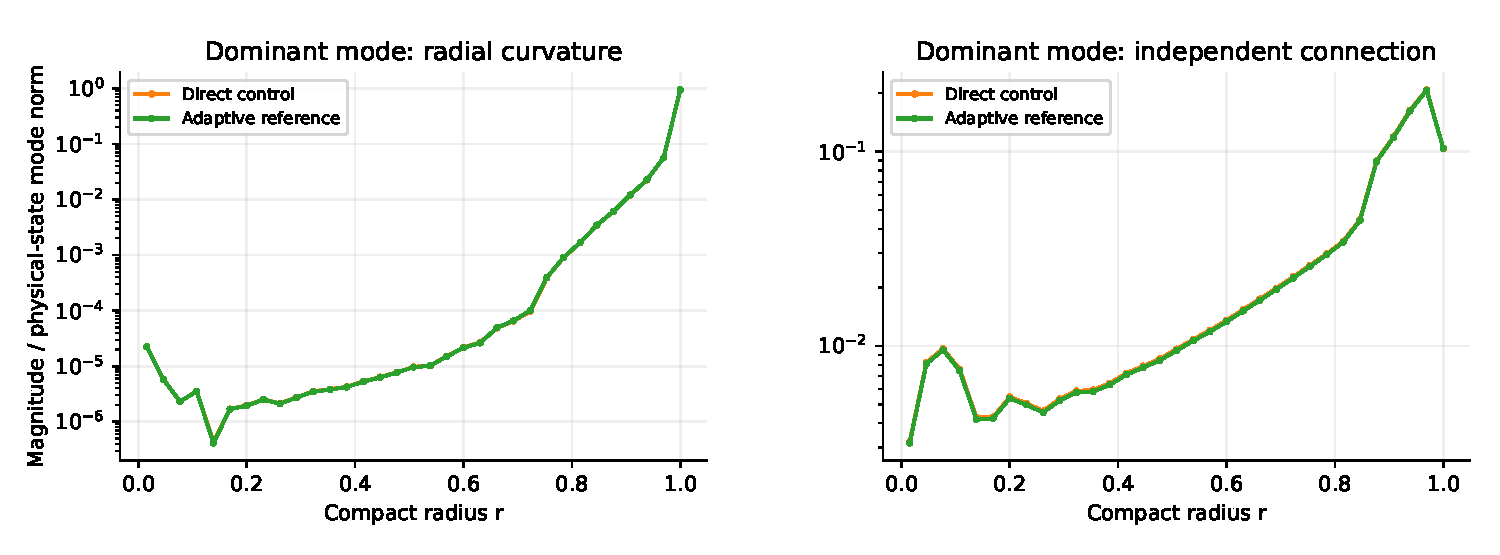
\includegraphics[width=\linewidth]{figures/boundary-mode.pdf}
\caption{Dominant modes at $N=33$, normalized by the norm of their physical-state entries. The independent endpoint derivative slots are excluded from that normalization. Curvature and connection components localize the growing mode in the outer region.}
\end{figure}

Diagnostic boundary-reduction relaxation strengths $1/h_{\rm scri}$ and $4/h_{\rm scri}$ barely reduce the dominant growth. Disabling the incoming-sensitive shear penalty alone also leaves growth. These controls do not qualify a repair and are not included in the frozen v1 trajectories. Reducing the timestep is assessed separately in the linearized map; its result is included below.
\FloatBarrier
\section{Trajectory outcomes and the advective comparison}

Trajectories use immutable source snapshots. Failed and bounded outcomes remain terminal; no failed state is restarted or relabeled. Crosses in the plots mark the last reported diagnostic, which can precede the actual failure time below. Table times are coordinate times; multiply by three to obtain $t/M$. The numerator guard is sampled approximately every $0.025$ coordinate-time units, so a reported stop is not an exact onset time.

\begin{center}\small\begin{tabular}{llrrl}\toprule

Candidate / test & $N$ & Target $t$ & Accepted $t$ & Outcome\\\midrule

Direct pulse & 65 & 0.1 & 0.1 & completed\\

Direct pulse & 65 & 1 & 0.223256 & failed\\

Direct puncture & 257 & 0.2 & 0.15 & failed\\

Adaptive pulse & 65 & 0.1 & 0.1 & completed\\

Adaptive pulse & 65 & 1 & 0.223256 & failed\\

Adaptive puncture & 257 & 0.2 & 0.15 & failed\\

Direct pulse & 129 & 1 & 0.224125 & failed\\

Adaptive pulse & 129 & 1 & 0.224125 & failed\\

\bottomrule\end{tabular}\end{center}

All 6 failed segments stop on the scri numerator guard. Their last accepted times and resolutions are retained in the table.

No candidate with a failed regular-center gate is promoted to a long puncture evolution. Consequently the $100M$ comparison, final-$20M$ drift fit for a new candidate, and a statement of improved late-time settling are unavailable. This is a failed qualification of the tested boundary implementation, not a measured puncture failure at $100M$ or a rejection of every discretization of the bulk equations.

The advective $N=257$ trajectory completes $100.0002M$. Its final relative horizon-mass error is $-2.563\times10^{-5}$, with peak sampled drift $1.655\times10^{-4}$. Its compact horizon radius changes from 0.062924 to 0.170409. The least-squares slope over $80.025$--$100.0002M$ is $9.306\times10^{-4}$ per unit $t/M$, with fit RMS $1.769\times10^{-4}$. Its final exterior mixed field-rate RMS is $9.073\times10^{-2}$. This surviving reference has not reached a stationary coordinate state by this diagnostic.

For the direct control puncture test, the last accepted time is $0.45M$. Peak sampled relative horizon-mass drift is $2.511\times10^{-9}$ and the last reported absolute relative mass error is $2.921\times10^{-9}$. There are 7 exact shared diagnostic times with the old history. The complete histories retain their native sample spacing; no unequal-time profile is used as a refinement comparison.

For the adaptive reference puncture test, the last accepted time is $0.45M$. Peak sampled relative horizon-mass drift is $2.509\times10^{-9}$ and the last reported absolute relative mass error is $2.919\times10^{-9}$. There are 7 exact shared diagnostic times with the old history. The complete histories retain their native sample spacing; no unequal-time profile is used as a refinement comparison.

At the latest exact shared diagnostic time, $t/M=0.45$, the direct control has the following finite-resolution comparison:

\begin{center}\small\begin{tabular}{lrrr}\toprule

Metric & New & Advective & New / old\\\midrule

Exterior H RMS & $1.424\times10^{-3}$ & $1.452\times10^{-3}$ & 0.9808\\

Exterior M RMS & $2.544\times10^{-2}$ & $2.811\times10^{-3}$ & 9.05\\

Exterior Theta RMS & $1.514\times10^{-5}$ & $5.025\times10^{-6}$ & 3.013\\

Exterior Z RMS & $1.619\times10^{-2}$ & $1.180\times10^{-4}$ & 137.2\\

\bottomrule\end{tabular}\end{center}

The compact horizon radii at this same time are 0.06478981 (new) and 0.06552123 (advective). This short comparison cannot establish a reduced late-time drift rate.

At the latest exact shared diagnostic time, $t/M=0.45$, the adaptive reference has the following finite-resolution comparison:

\begin{center}\small\begin{tabular}{lrrr}\toprule

Metric & New & Advective & New / old\\\midrule

Exterior H RMS & $1.425\times10^{-3}$ & $1.452\times10^{-3}$ & 0.981\\

Exterior M RMS & $2.440\times10^{-2}$ & $2.811\times10^{-3}$ & 8.681\\

Exterior Theta RMS & $1.471\times10^{-5}$ & $5.025\times10^{-6}$ & 2.927\\

Exterior Z RMS & $1.554\times10^{-2}$ & $1.180\times10^{-4}$ & 131.7\\

\bottomrule\end{tabular}\end{center}

The compact horizon radii at this same time are 0.06479176 (new) and 0.06552123 (advective). This short comparison cannot establish a reduced late-time drift rate.

\clearpage\subsection{Diagnostic plots}

\begin{figure}[htbp]\centering

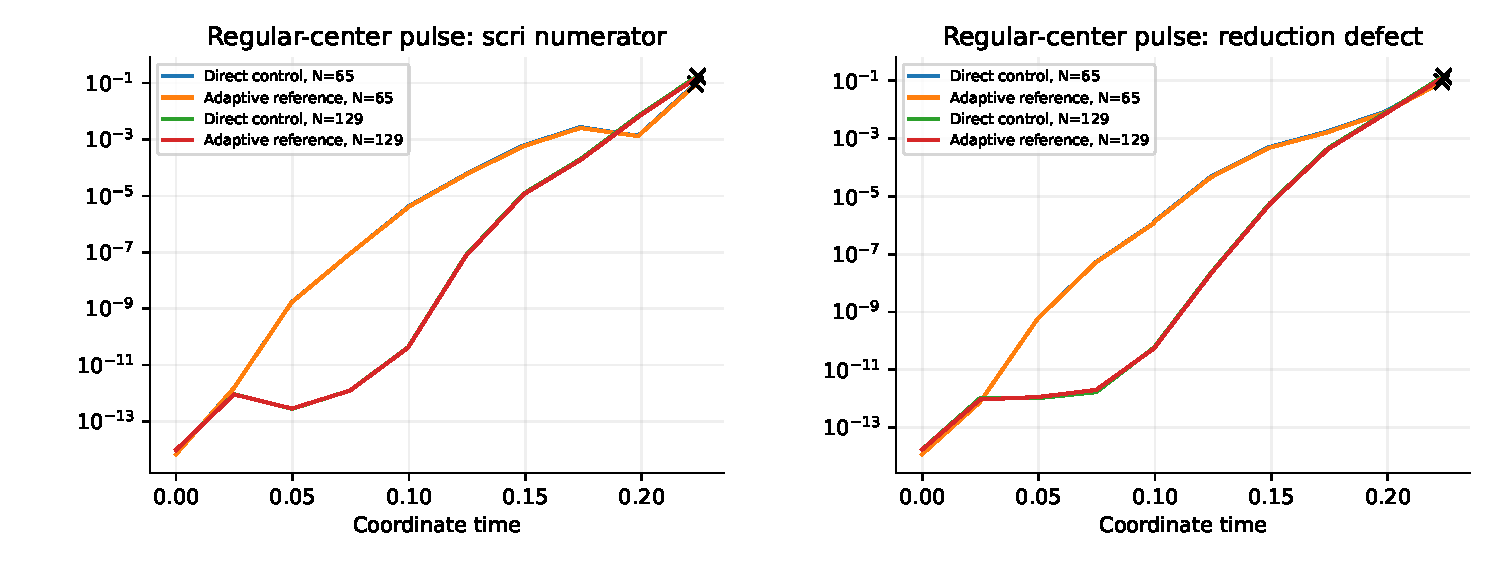
\includegraphics[width=\linewidth]{figures/pulse-gates.pdf}

\caption{Regular-center pulse gates, in coordinate time. The numerator and derivative-reduction defects expose boundary growth separately from exact nullness.}\end{figure}

\begin{figure}[htbp]\centering

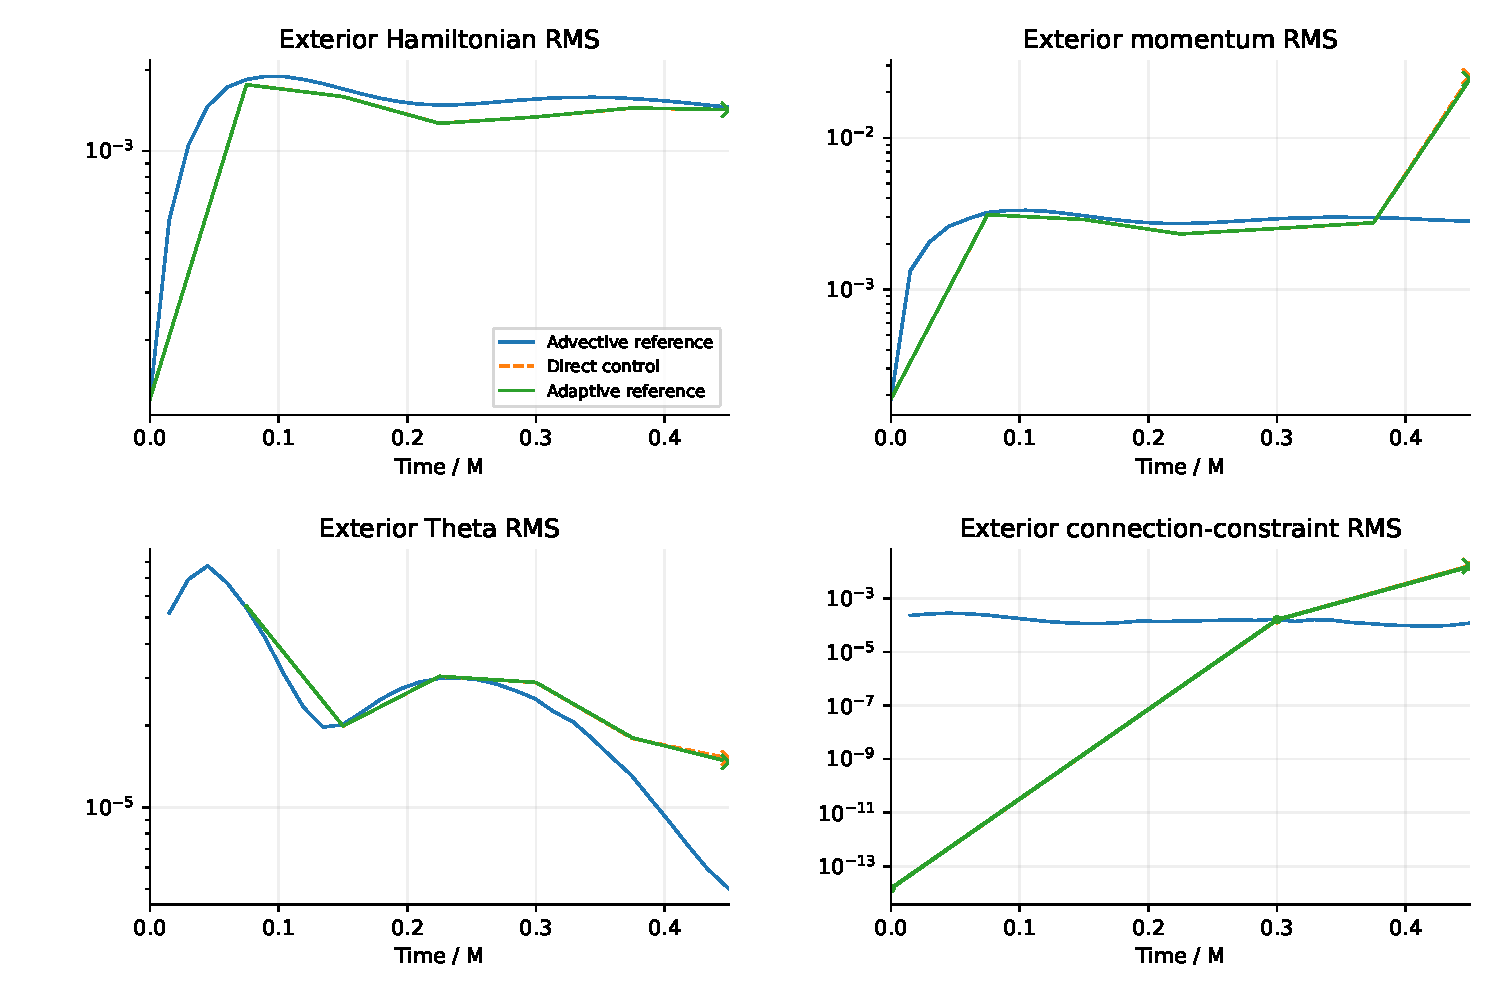
\includegraphics[width=\linewidth]{figures/exterior-constraints.pdf}

\caption{Apparent-horizon-exterior RMS Hamiltonian, momentum, Theta, and connection constraints. The primary Z curves use independent metric finite differences on saved profiles and terminal states; the other three diagnostics agree with the independently recomputed values there. Norms are normalized over exterior radial weights. Zero values are omitted only on logarithmic axes.}\end{figure}

\begin{figure}[htbp]\centering

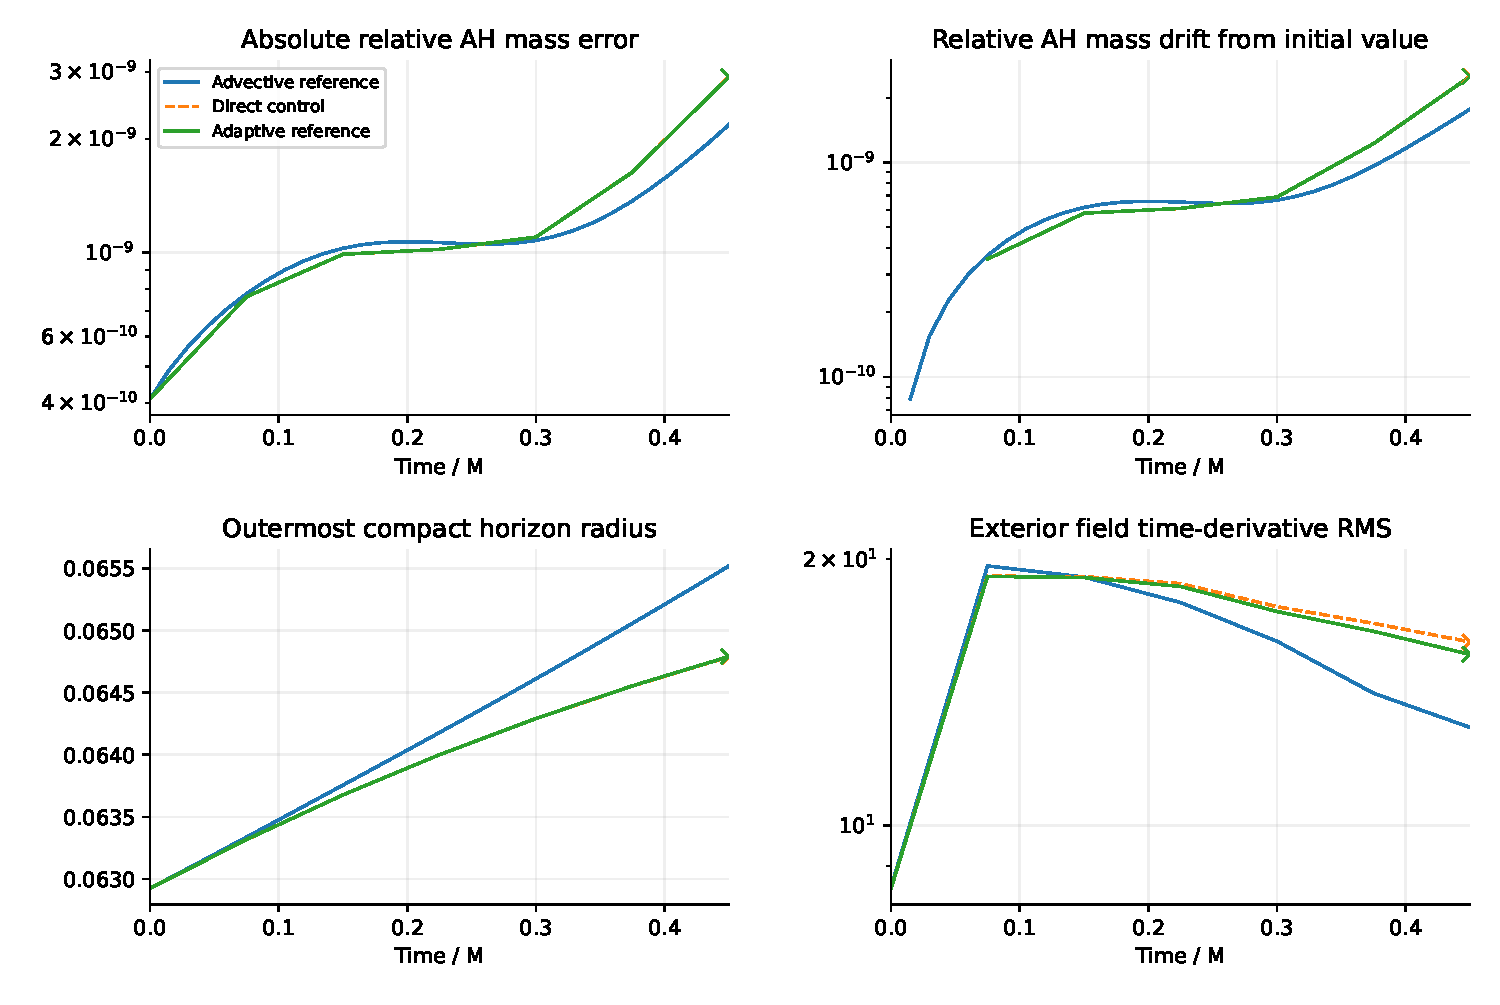
\includegraphics[width=\linewidth]{figures/mass-horizon-settling.pdf}

\caption{Outermost-horizon mass error, drift from each numerical initial mass, compact horizon radius, and candidate field-rate RMS. The time window shows the actual short candidate evidence; it does not imply a late-time comparison. Reference field rates at the short common times come from read-only diagnostics on the exactly recovered sampling replay; its 100M value is reported separately.}\end{figure}

\begin{figure}[htbp]\centering

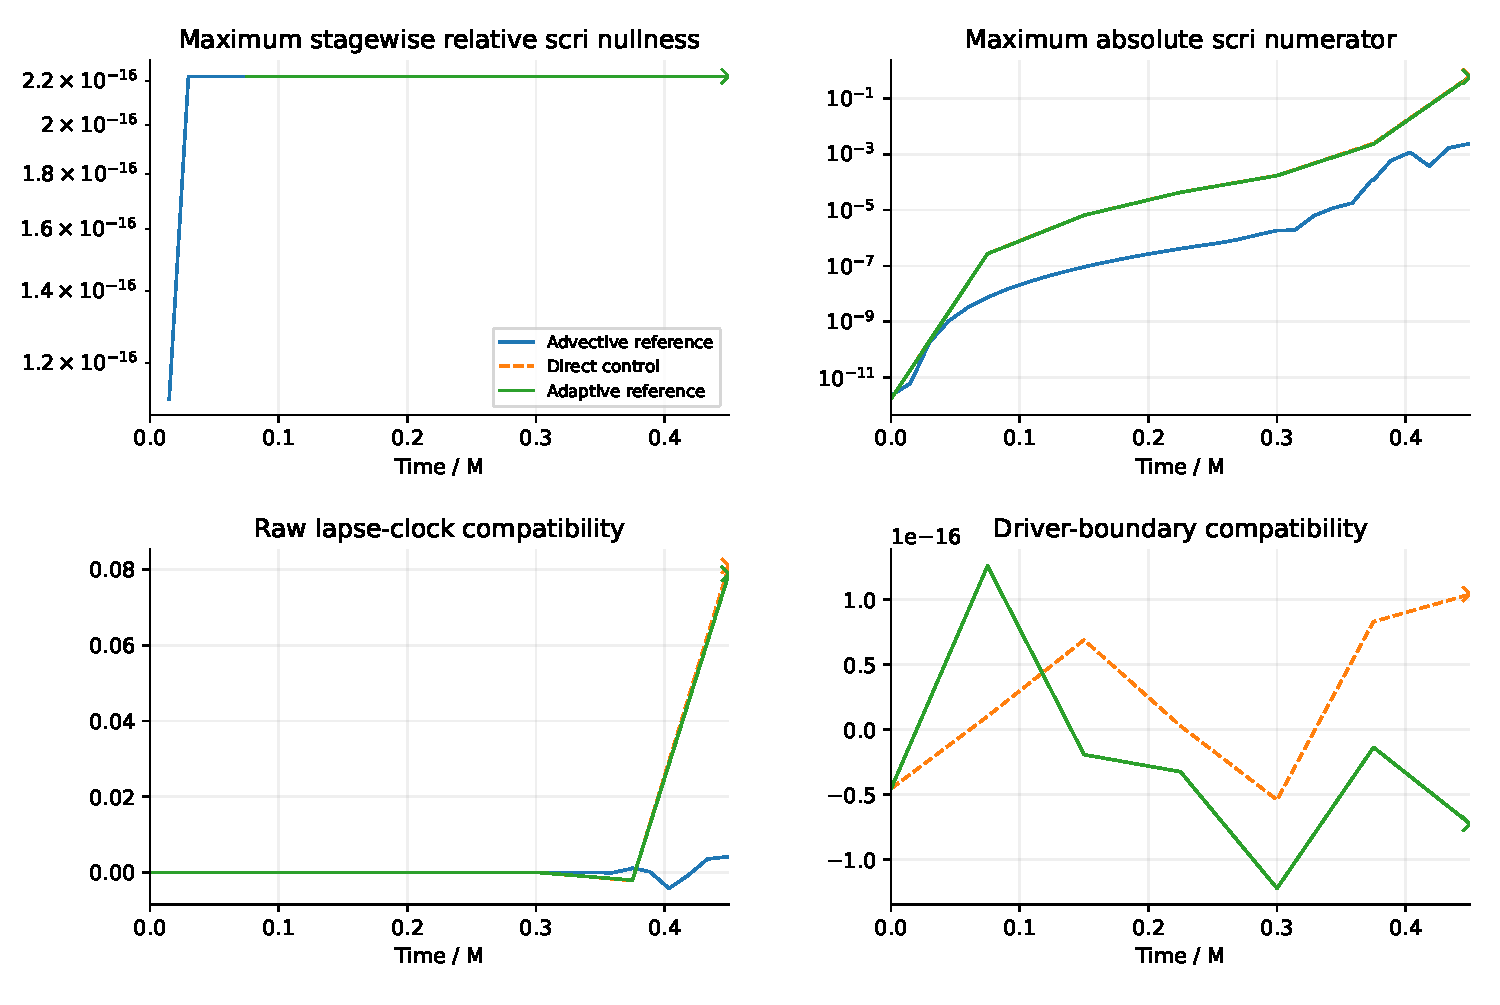
\includegraphics[width=\linewidth]{figures/boundary-health.pdf}

\caption{Maximum stagewise relative nullness, current numerator residual, raw lapse-clock compatibility, and the new driver compatibility residual. Roundoff gauge identities can coexist with growing regularity errors.}\end{figure}

\begin{figure}[htbp]\centering

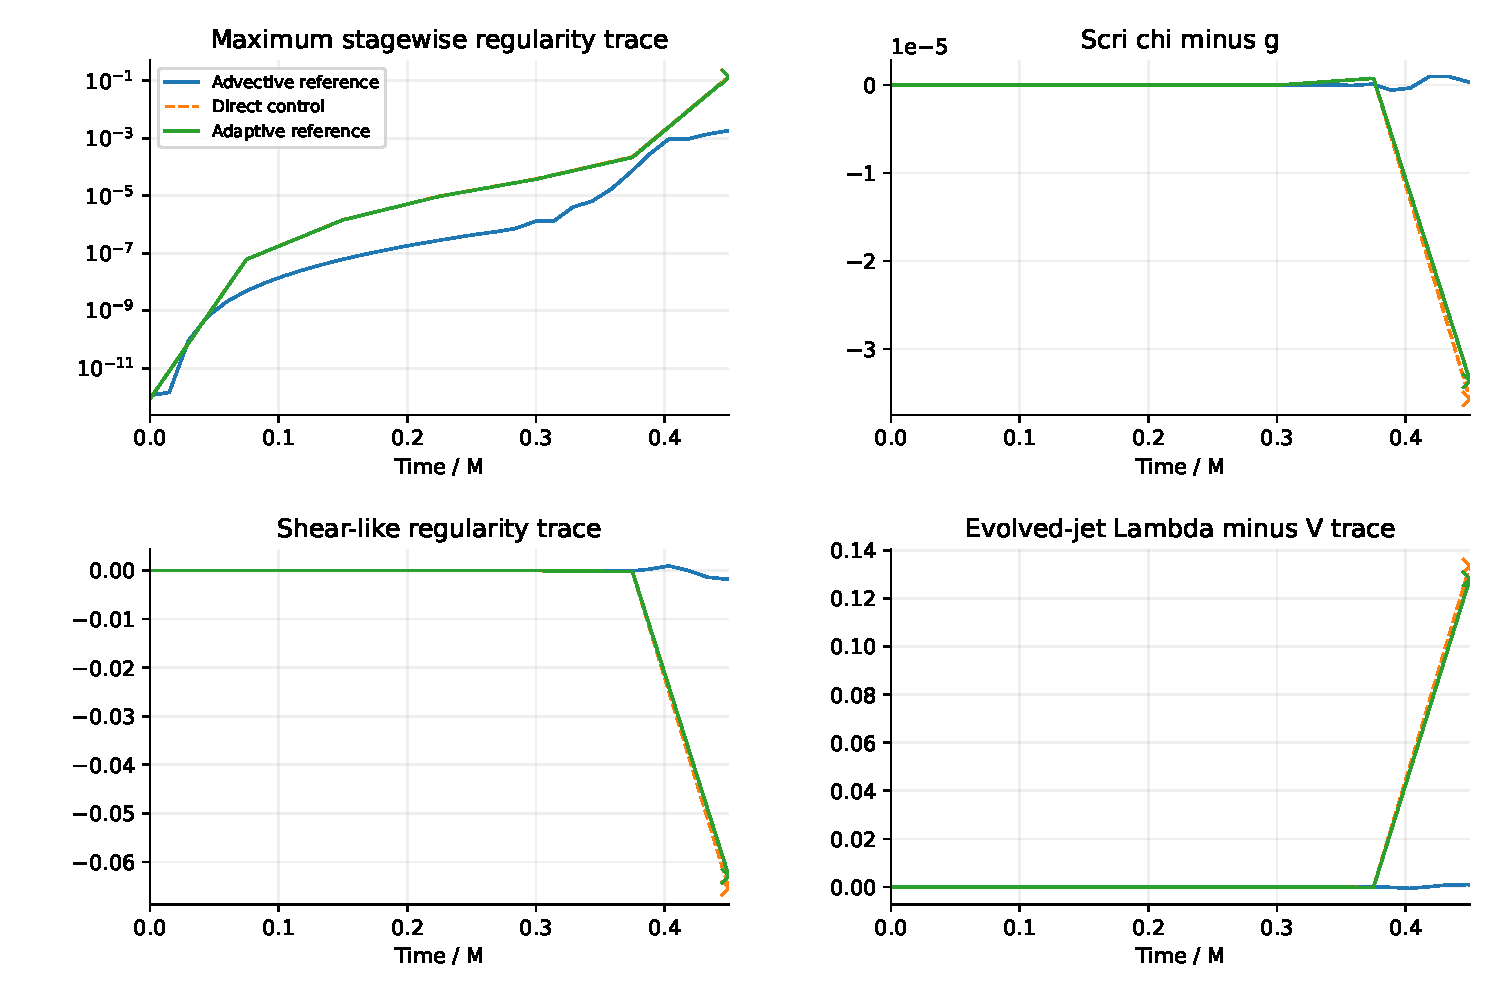
\includegraphics[width=\linewidth]{figures/regularity-traces.pdf}

\caption{Approximate regularity traces, distinct from exact nullness. These use the evolved boundary jet, whose inconsistency with metric reconstruction is quantified separately.}\end{figure}

\begin{figure}[htbp]\centering

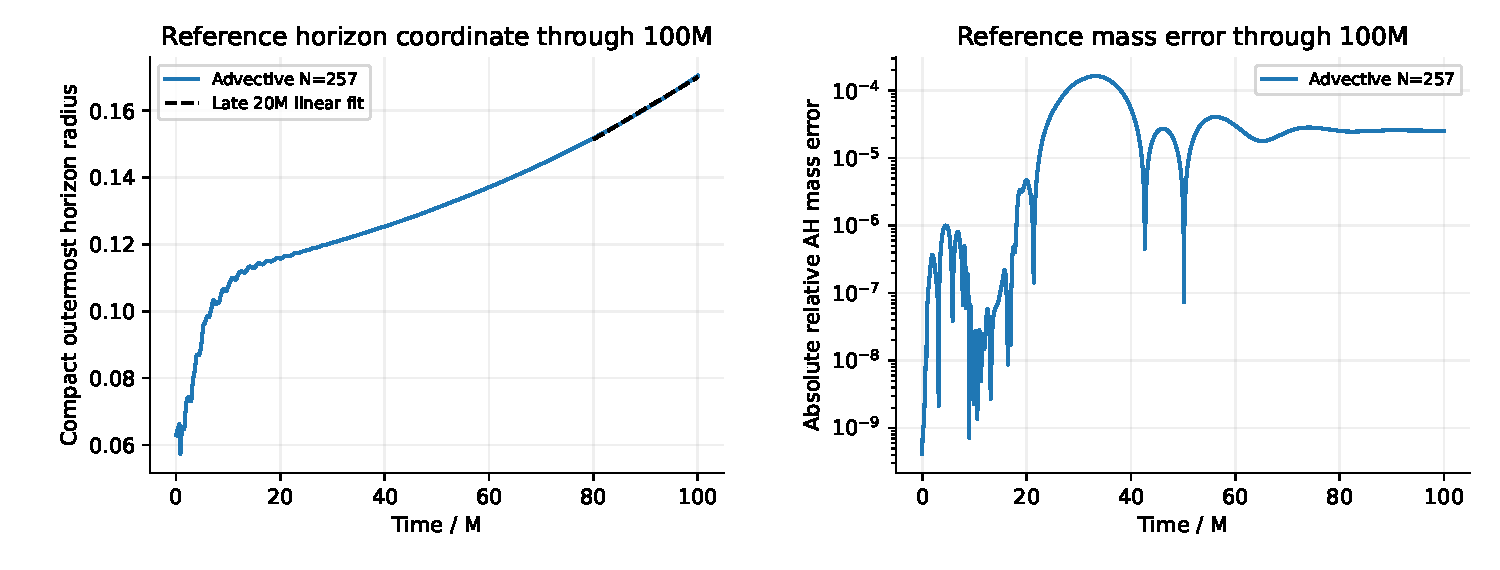
\includegraphics[width=\linewidth]{figures/advective-duration-context.pdf}

\caption{The preserved advective duration context. The late horizon-coordinate fit uses the final $20M$; no new candidate reaches this interval. Short matched new profiles and histories are shown separately.}\end{figure}

\begin{figure}[htbp]\centering

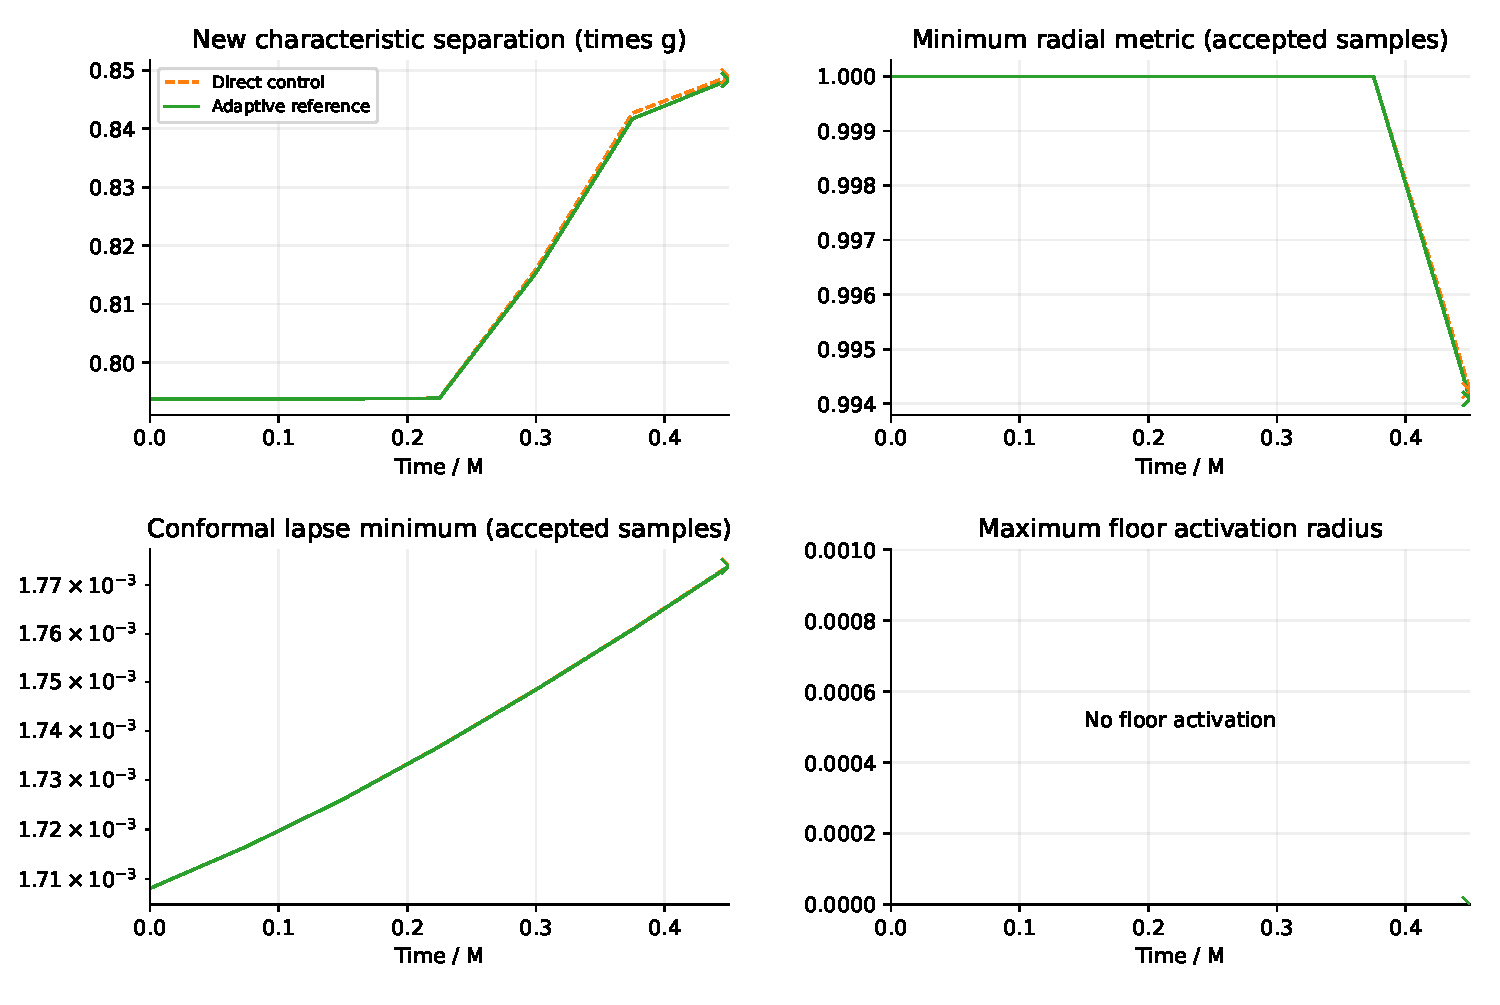
\includegraphics[width=\linewidth]{figures/gauge-positivity-floor.pdf}

\caption{New sufficient characteristic-separation margin, geometry minima at accepted diagnostic samples, and maximum stage floor radius. The old advective gap has a different definition and is not superposed.}\end{figure}

\begin{figure}[htbp]\centering

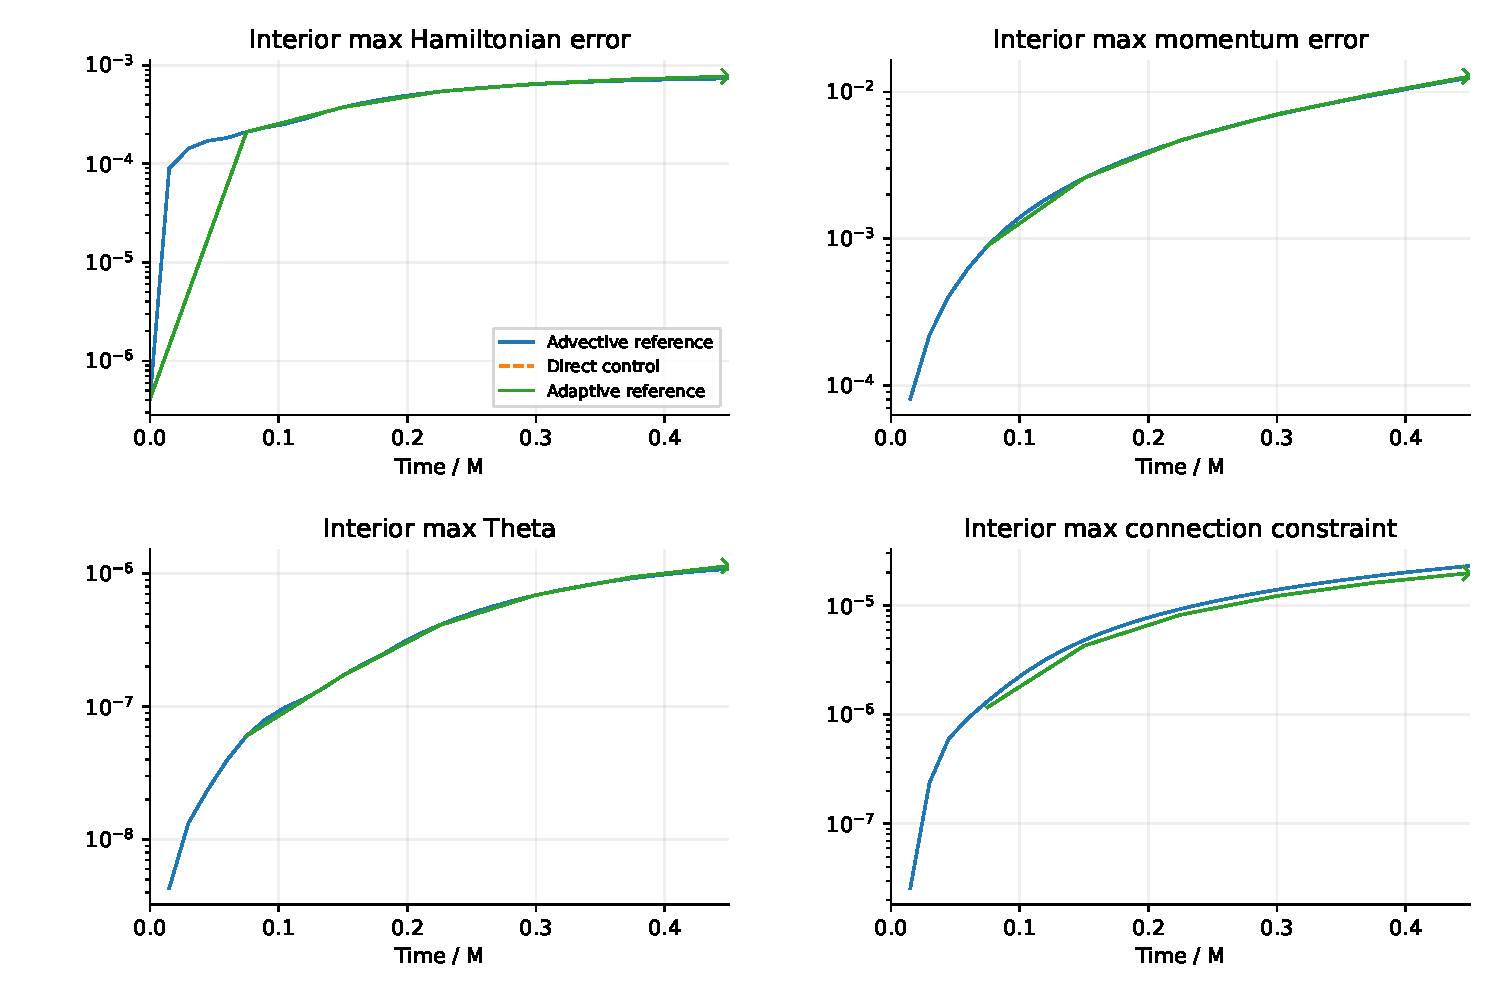
\includegraphics[width=\linewidth]{figures/interior-errors.pdf}

\caption{Interior constraint errors are retained separately and do not enter the exterior accuracy budget. No positive-radius neighborhood has been silently removed.}\end{figure}

\begin{figure}[htbp]\centering

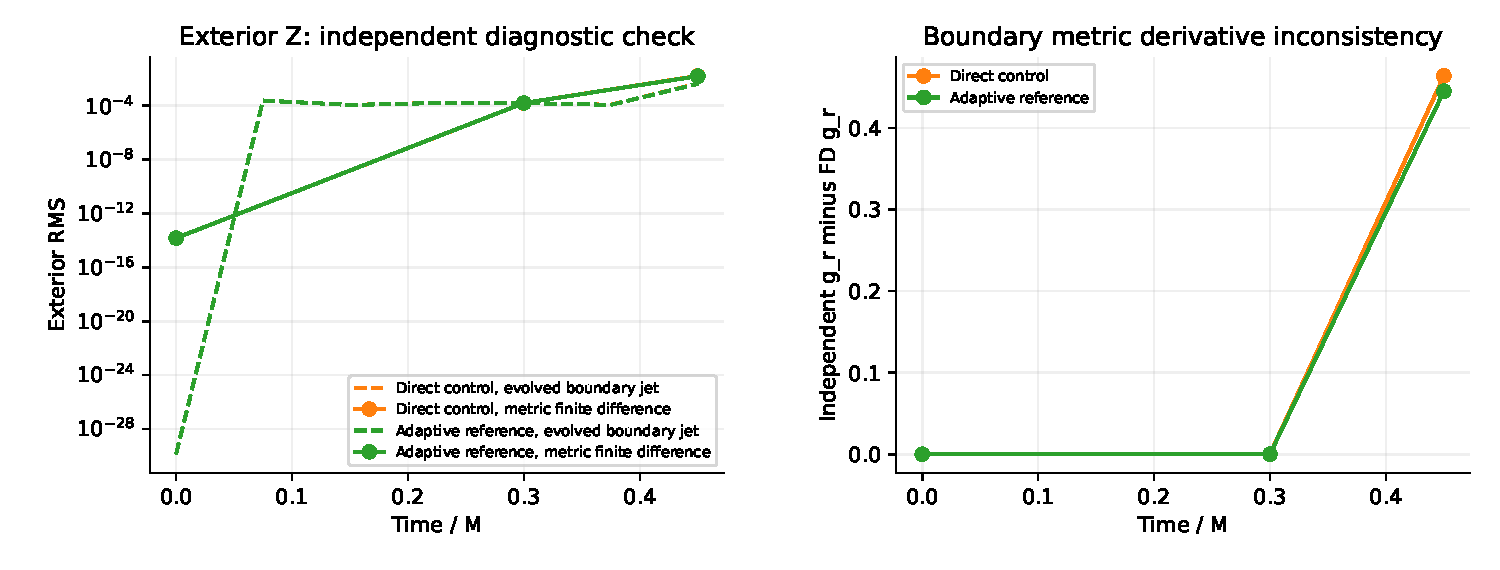
\includegraphics[width=\linewidth]{figures/constraint-definition.pdf}

\caption{The independent constraint-definition audit. Dashed curves use evolved boundary jets; solid markers reconstruct the derivative from metric values. Their difference exposes the reduction-consistency failure instead of suppressing its endpoint contribution.}\end{figure}

\begin{figure}[htbp]\centering

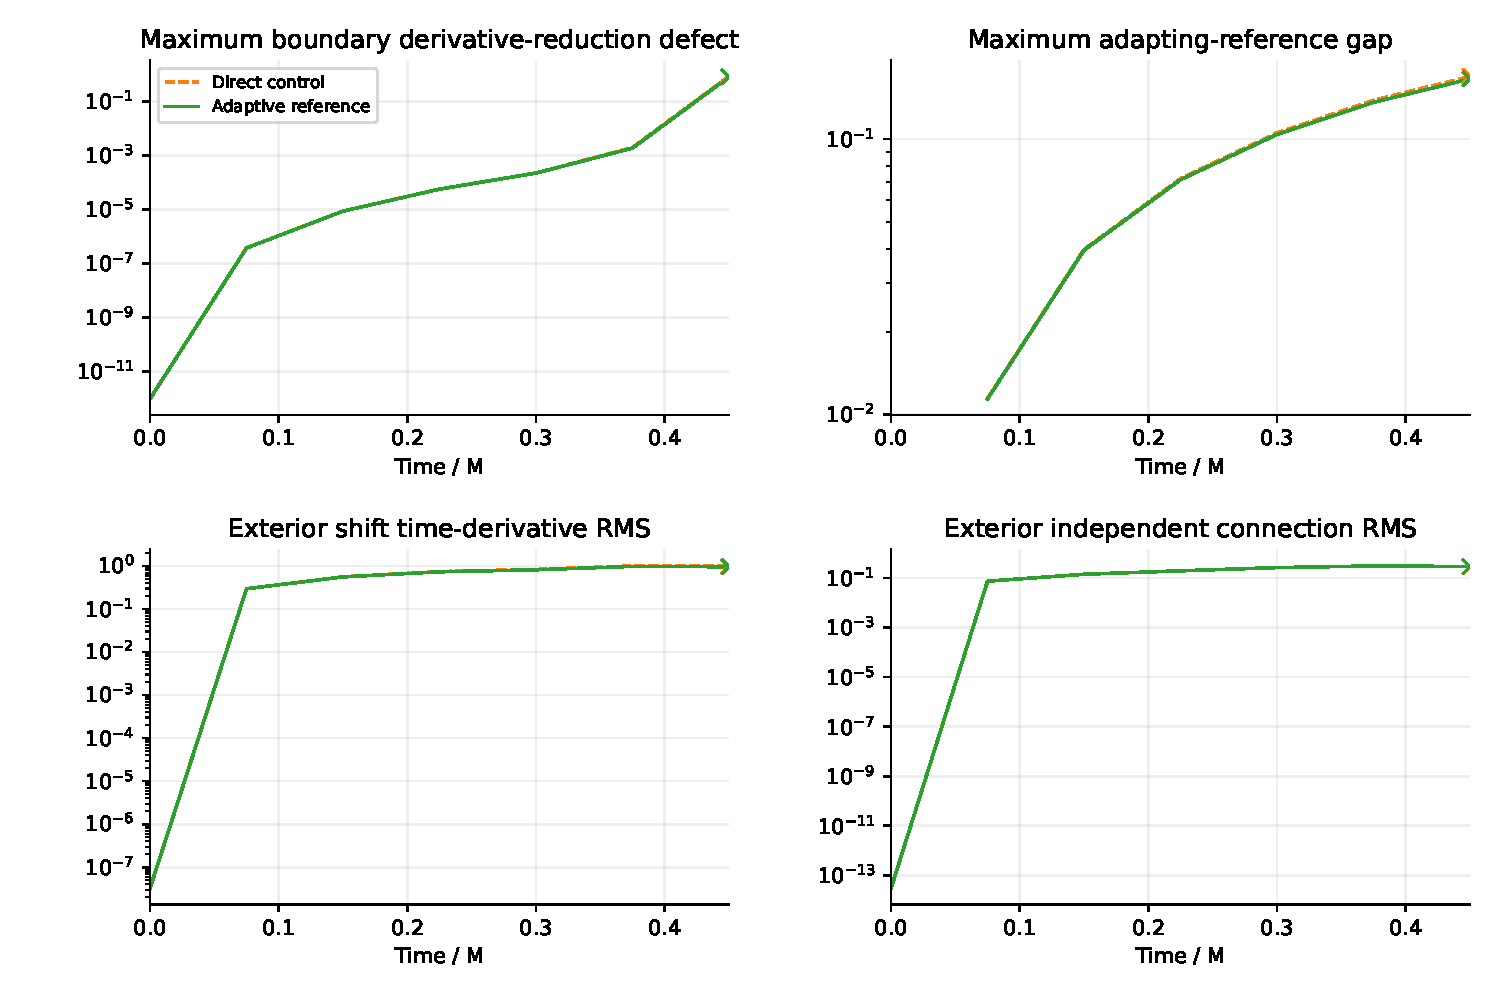
\includegraphics[width=\linewidth]{figures/reduction-and-settling.pdf}

\caption{Boundary derivative-reduction defects, reference gap, shift rate, and independent connection residual. These distinguish coordinate settling from simple horizon-radius flattening.}\end{figure}

\begin{figure}[htbp]\centering

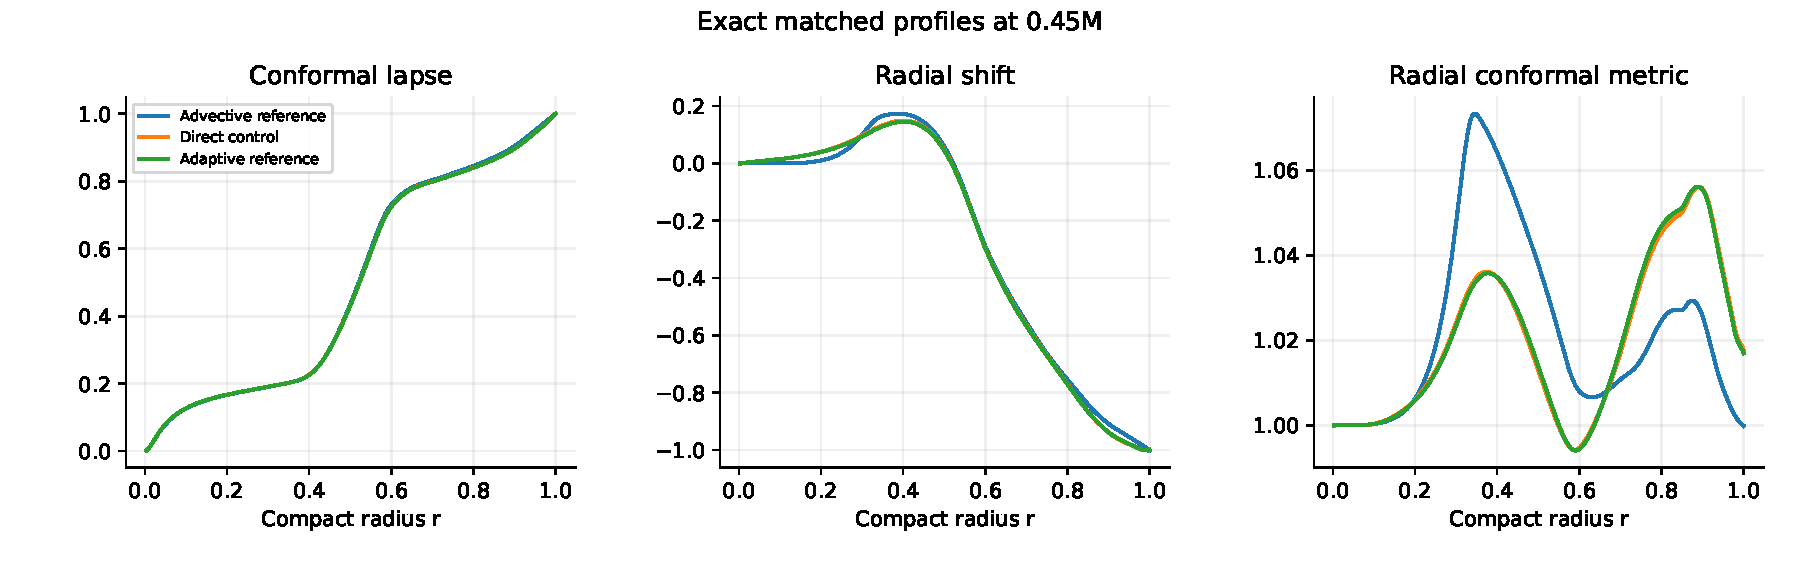
\includegraphics[width=\linewidth]{figures/matched-profiles.pdf}

\caption{Lapse, shift, and radial metric at an exact common saved time. Every positive-radius node is retained; the central coefficient endpoint is not a physical puncture sample.}\end{figure}

\FloatBarrier\subsection{Boundary timestep and diagnostic checks}

For the direct control at $N=33$, halving the timestep changes the dominant growth rate from 11.40269 to 11.40269 per unit coordinate time. The growing frozen mode therefore persists under this timestep reduction; the result is not explained by a large RK step alone.

For the adaptive control at $N=33$, halving the timestep changes the dominant growth rate from 10.86828 to 10.86828 per unit coordinate time. The growing frozen mode therefore persists under this timestep reduction; the result is not explained by a large RK step alone.

An independent recomputation of the native constraints replaces the evolved endpoint derivative reductions by ordinary finite-difference derivatives on every saved profile and last accepted state. Maximum changes in the H, M, Theta, and Z diagnostics are respectively $0,\ 0,\ 0,\ 2.278\times10^{-1}$. The Z difference is material and the metric-reconstructed Z norm is therefore used for the primary comparison. This exposes the boundary consistency failure; it does not repair the evolution.

\subsection{Answers to the comparison questions}

The tested implementation has no qualified $100M$ result. Reduced late-time horizon drift and competitive long-time exterior constraints or mass conservation are therefore unestablished. Exact nullness is assessed on the actual evaluated stages, not extrapolated to an unperformed long run. The numerical boundary growth prevents a claim of improved settling or robustness. No nearby reference-rate scan is justified by a failure already localized in the boundary discretization.


\section{Implication for a subsequent boundary attempt}
A possible next implementation is a consistent first-order reduction through an outer collar, or a ghost construction whose derivatives are consistent with the same metric values. It would need to impose the single incoming gauge relation while preserving the physical outgoing constraint fields, and test that preservation before long evolution. The present independent-endpoint-jet construction does not meet that requirement. Varying the reference relaxation rate does not address the diagnosed consistency defect.

\section{Reproducibility and assessment limits}
The experiment is isolated on \texttt{codex/nonadvective-adaptive-reference}. Inputs and comparison criteria are under \path{inputs/nonadvective_shift_1d/}; implementation and analysis tools are under \path{tst/nonadvective_shift_1d/}. Each trajectory binds frozen sources, the native library, numerical parameters, and checkpoint hashes. Continuations require a verified completed parent. Every integration segment is capped at 420 seconds; failures and bounded stops are terminal and retain their actual outcomes. The controller reserves the existing main-thread slots through serial child transitions and permits at most two simultaneous evolution processes.

Finite-error radial-weighted constraint norms are gauge dependent; apparent-horizon mass supplies the invariant comparison. Exterior RMS norms use only nodes outside the outermost apparent horizon and normalize by the exterior radial weights. Interior errors are retained and plotted separately. No physical positive-radius node is excised. Unequal terminal times are not treated as a refinement test, and a single surviving low-resolution run cannot establish convergence. A failure of this boundary discretization does not by itself reject every possible implementation of the proposed nonadvective bulk gauge.
\end{document}
